\section{hpgs\_\-paint\_\-clipper\_\-st Struct Reference}
\label{structhpgs__paint__clipper__st}\index{hpgs\_\-paint\_\-clipper\_\-st@{hpgs\_\-paint\_\-clipper\_\-st}}
A collection of scanlines for mapping paths onto images.  


{\tt \#include $<$hpgspaint.h$>$}

\subsection*{Data Fields}
\begin{CompactItemize}
\item 
{\bf hpgs\_\-bbox} \textbf{bb}\label{structhpgs__paint__clipper__st_99e473a73883b3dc7f878011ccc78a29}

\item 
hpgs\_\-bool {\bf overscan}
\item 
int {\bf height}
\item 
int {\bf iscan0}
\item 
int {\bf iscan1}
\end{CompactItemize}
\begin{Indent}{\bf }\par
\begin{CompactItemize}
\item 
{\bf hpgs\_\-paint\_\-scanline} $\ast$ {\bf scanlines}
\item 
int \textbf{n\_\-scanlines}\label{structhpgs__paint__clipper__st_367b1a282fe5383aa5f263180c804fcc}

\end{CompactItemize}
\end{Indent}
\begin{Indent}{\bf }\par
\begin{CompactItemize}
\item 
double {\bf yfac}
\item 
double \textbf{y0}\label{structhpgs__paint__clipper__st_40c3cba1b7385c968894c9c22eb914cb}

\end{CompactItemize}
\end{Indent}


\subsection{Detailed Description}
A collection of scanlines for mapping paths onto images. 

This structure has a public alias {\tt hpgs\_\-paint\_\-clipper} and holds intersection points of a path with a rectangular region represented by a series of equidistantly distributed scanlines.

The {\tt overscan} member determines, whether we use antialiasing for mappinng the path. The name of this structure member is historical, because up to {\tt hpgs-0.8.x} the antialiasing renderer effectively used more than one scanline per physical image row in order to caclulate alpha values.

Nowadays a scanline always represents the middle of the corresponding physical row of the image as sketch in the folowing figure, which show the generated segment for non-antialiased rendering.

 \begin{Image}
\begin{center}
\includegraphics{scanline_0}\caption{scanline setup and pixel filling without antialiasing.}
\end{center}
\end{Image}
 If {\tt overscan} is non-zero, the segment generator caclulates slopes of the trapezoids, which are generated by the path segments cutting the boundaries between two physical grid lines as sketched in the following figure.

 \begin{Image}
\begin{center}
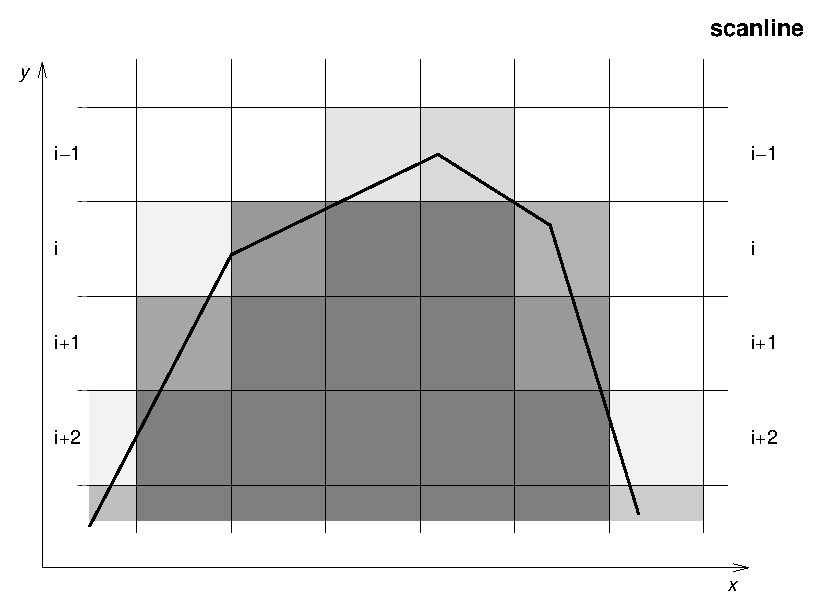
\includegraphics{scanline_n}\caption{scanline setup and alpha generation with antialiasing.}
\end{center}
\end{Image}


\subsection{Field Documentation}
\index{hpgs\_\-paint\_\-clipper\_\-st@{hpgs\_\-paint\_\-clipper\_\-st}!scanlines@{scanlines}}
\index{scanlines@{scanlines}!hpgs_paint_clipper_st@{hpgs\_\-paint\_\-clipper\_\-st}}
\subsubsection[scanlines]{\setlength{\rightskip}{0pt plus 5cm}{\bf hpgs\_\-paint\_\-scanline}$\ast$ {\bf hpgs\_\-paint\_\-clipper\_\-st::scanlines}}\label{structhpgs__paint__clipper__st_0bb91ce08576e1de31698acf4edb5a53}


The vector of scanlines in this clipper. 

Referenced by hpgs\_\-new\_\-paint\_\-clipper(), hpgs\_\-paint\_\-clipper\_\-clear(), hpgs\_\-paint\_\-clipper\_\-clip(), hpgs\_\-paint\_\-clipper\_\-destroy(), hpgs\_\-paint\_\-clipper\_\-emit(), hpgs\_\-paint\_\-clipper\_\-reset(), hpgs\_\-paint\_\-clipper\_\-thin\_\-cut(), and hpgs\_\-paint\_\-device\_\-drawimage().\index{hpgs\_\-paint\_\-clipper\_\-st@{hpgs\_\-paint\_\-clipper\_\-st}!yfac@{yfac}}
\index{yfac@{yfac}!hpgs_paint_clipper_st@{hpgs\_\-paint\_\-clipper\_\-st}}
\subsubsection[yfac]{\setlength{\rightskip}{0pt plus 5cm}double {\bf hpgs\_\-paint\_\-clipper\_\-st::yfac}}\label{structhpgs__paint__clipper__st_0cdd33a5c1f522e1445d74fd18ec2da2}


The bounding box of this clipper in world coordinates.

The mapping of scanline numbers to world coordinates. {\tt iscan=}(y0-y)/yfac and {\tt y=y0-iscan$\ast$yfac}. 

Referenced by hpgs\_\-new\_\-paint\_\-clipper(), and hpgs\_\-paint\_\-device\_\-drawimage().\index{hpgs\_\-paint\_\-clipper\_\-st@{hpgs\_\-paint\_\-clipper\_\-st}!overscan@{overscan}}
\index{overscan@{overscan}!hpgs_paint_clipper_st@{hpgs\_\-paint\_\-clipper\_\-st}}
\subsubsection[overscan]{\setlength{\rightskip}{0pt plus 5cm}hpgs\_\-bool {\bf hpgs\_\-paint\_\-clipper\_\-st::overscan}}\label{structhpgs__paint__clipper__st_b0fe1dce067b9c2fdbceb38bbe496e02}


Do we use antialiasing ?. 

Referenced by hpgs\_\-new\_\-paint\_\-clipper(), hpgs\_\-paint\_\-clipper\_\-clip(), hpgs\_\-paint\_\-clipper\_\-cut(), hpgs\_\-paint\_\-clipper\_\-emit(), and hpgs\_\-paint\_\-clipper\_\-reset().\index{hpgs\_\-paint\_\-clipper\_\-st@{hpgs\_\-paint\_\-clipper\_\-st}!height@{height}}
\index{height@{height}!hpgs_paint_clipper_st@{hpgs\_\-paint\_\-clipper\_\-st}}
\subsubsection[height]{\setlength{\rightskip}{0pt plus 5cm}int {\bf hpgs\_\-paint\_\-clipper\_\-st::height}}\label{structhpgs__paint__clipper__st_86d0fcb90e48b744eeb3ac6ffcb287ed}


Number of physical pixels of the underlying image. 

Referenced by hpgs\_\-new\_\-paint\_\-clipper(), hpgs\_\-paint\_\-clipper\_\-clip(), and hpgs\_\-paint\_\-clipper\_\-emit().\index{hpgs\_\-paint\_\-clipper\_\-st@{hpgs\_\-paint\_\-clipper\_\-st}!iscan0@{iscan0}}
\index{iscan0@{iscan0}!hpgs_paint_clipper_st@{hpgs\_\-paint\_\-clipper\_\-st}}
\subsubsection[iscan0]{\setlength{\rightskip}{0pt plus 5cm}int {\bf hpgs\_\-paint\_\-clipper\_\-st::iscan0}}\label{structhpgs__paint__clipper__st_23f85f972d3629d30f8f032640d4b77e}


The first scanline with non-zero intersections. 

Referenced by hpgs\_\-new\_\-paint\_\-clipper(), hpgs\_\-paint\_\-clipper\_\-clear(), hpgs\_\-paint\_\-clipper\_\-clip(), hpgs\_\-paint\_\-clipper\_\-emit(), hpgs\_\-paint\_\-clipper\_\-reset(), hpgs\_\-paint\_\-clipper\_\-thin\_\-cut(), and hpgs\_\-paint\_\-device\_\-drawimage().\index{hpgs\_\-paint\_\-clipper\_\-st@{hpgs\_\-paint\_\-clipper\_\-st}!iscan1@{iscan1}}
\index{iscan1@{iscan1}!hpgs_paint_clipper_st@{hpgs\_\-paint\_\-clipper\_\-st}}
\subsubsection[iscan1]{\setlength{\rightskip}{0pt plus 5cm}int {\bf hpgs\_\-paint\_\-clipper\_\-st::iscan1}}\label{structhpgs__paint__clipper__st_c2711333e8f5dfc95b6a33f0c4954b6f}


The last scanline with non-zero intersections. 

Referenced by hpgs\_\-new\_\-paint\_\-clipper(), hpgs\_\-paint\_\-clipper\_\-clear(), hpgs\_\-paint\_\-clipper\_\-clip(), hpgs\_\-paint\_\-clipper\_\-emit(), hpgs\_\-paint\_\-clipper\_\-reset(), and hpgs\_\-paint\_\-device\_\-drawimage().

The documentation for this struct was generated from the following file:\begin{CompactItemize}
\item 
{\bf hpgspaint.h}\end{CompactItemize}
